\documentclass[conference]{IEEEtran}
\IEEEoverridecommandlockouts
% The preceding line is only needed to identify funding in the first footnote. If that is unneeded, please comment it out.
\usepackage{cite}
\usepackage{amsmath,amssymb,amsfonts}
\usepackage{graphicx}
\usepackage{textcomp}
\usepackage{xcolor}
\def\BibTeX{{\rm B\kern-.05em{\sc i\kern-.025em b}\kern-.08em
    T\kern-.1667em\lower.7ex\hbox{E}\kern-.125emX}}
\title{
\vspace{1cm}
{
\includegraphics[width=0.15\textwidth]{ /storage/emulated/0/FWC1/fpga/IMG-20241021-WA0004.jpg} \\ FPGA Assignment} }
\author{Sivva Pranaykumar\\ Roll No: FWC22273\\ sivvapranay.s@gmail.com}
 \begin{document}
\maketitle
 \section {ABSTRACT}
A 4-bit priority encoder has inputs D3, D2, D1 and D0 in descending order of priority. The two-bit output AB is generated as 00, 01, 10 and 11 corresponding to inputs D3, D2, D1 and D0, respectively. The Boolean expression of the output bit B is to be implemented.
\section{COMPONENTS}
The required components list is given in Table: I. 

\begin{figure}[h]
\centering
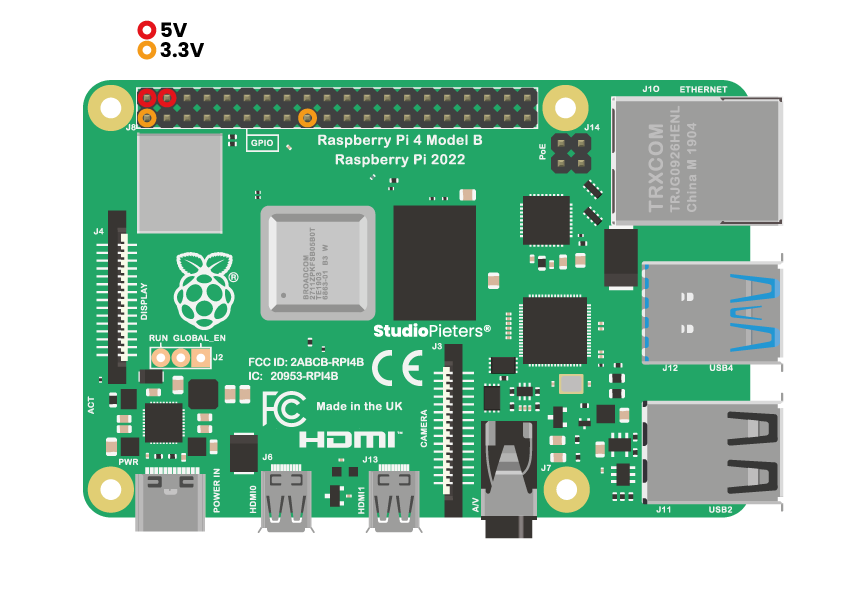
\includegraphics[width=0.4\textwidth]{/storage/emulated/0/FWC1/fpga/17313068981125684858793623388663.png         }    
\end{figure}

 \begin {figure} [h]
 \centering
 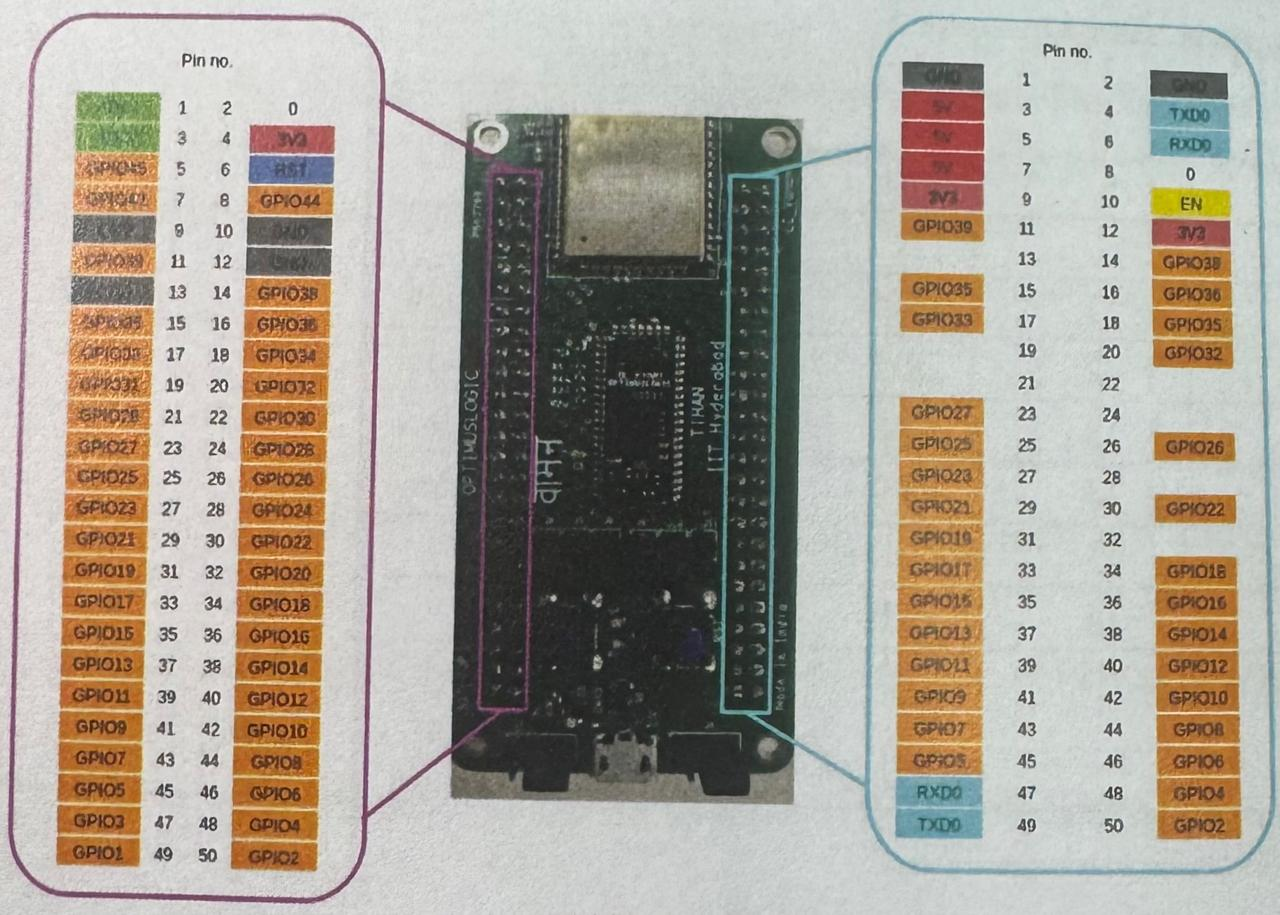
\includegraphics[width=0.35\textwidth]{/storage/emulated/0/FWC1/fpga/IMG-20241024-WA0005.jpg        }
 \end {figure}

\begin{table} [htbp]
\centering
\begin{tabular}{| c | c | c |} \hline
Components & Value & Quantity \\\hline
Rasberry Pi &  & 1 \\\hline
Vaman Board&  & 1 \\\hline
SD card&  & 1 \\\hline
LEDs &  & 1 \\ \hline
Jumper Wires &  & 10 \\ \hline
Breadboard & & 1 \\ 
\hline
\end{tabular}
\vspace{0.1cm}
\caption{\label{tab:widgets}}
\end{table}
\section{PROCEDURE}
To set up the circuit, first connect the input pins D0, D1, D2, and D3 to GPIO pins on the pygm board and connect the output pin B to an LED or other output device. Use the appropriate programming environment (Python for Raspberry Pi or C/C++ for the pygm board) to configure the input pins as inputs and the B pin as an output. Implement the Boolean logic expression $B={\bar{D3}}D2+{\bar{D3}} {\bar{D1}}$ in your code, continuously reading the inputs and updating the output. Power on the system, run the program, and test various combinations of inputs (VCC or GND) according to the truth table, observing the output (LED on/off) to verify the correct operation of the circuit.
\begin{table} [htbp]
\centering
\begin{tabular}{| c | c | c | c | c | c |} \hline
D3& D2& D1& D0& A & B  \\\hline
1 & x & x & x & 0 & 0\\ \hline
0 & 1 & x & x & 0 & 1\\ \hline
0 & 0 & 1 & x & 1 & 0\\ \hline
0 & 0 & 0 & 1 & 1 & 1 \\ \hline

\end{tabular}
\vspace{0.2cm}
\caption{\label{tab:widgets}}
\end{table}

\section{RESULTS}
The project successfully implemented the Boolean logic circuit, where the system correctly read inputs D3, D2, D1, and D0 and applied the expression $B={\bar{D3}}D2+{\bar{D3}} {\bar{D1}}$ to determine the output. The LED controlled by pin B turned on or off based on the truth table conditions, confirming the correct functionality of the circuit. The consistent behavior validated the proper implementation of the Boolean logic on both the Raspberry Pi and pygm board.


\begin{figure}[h]
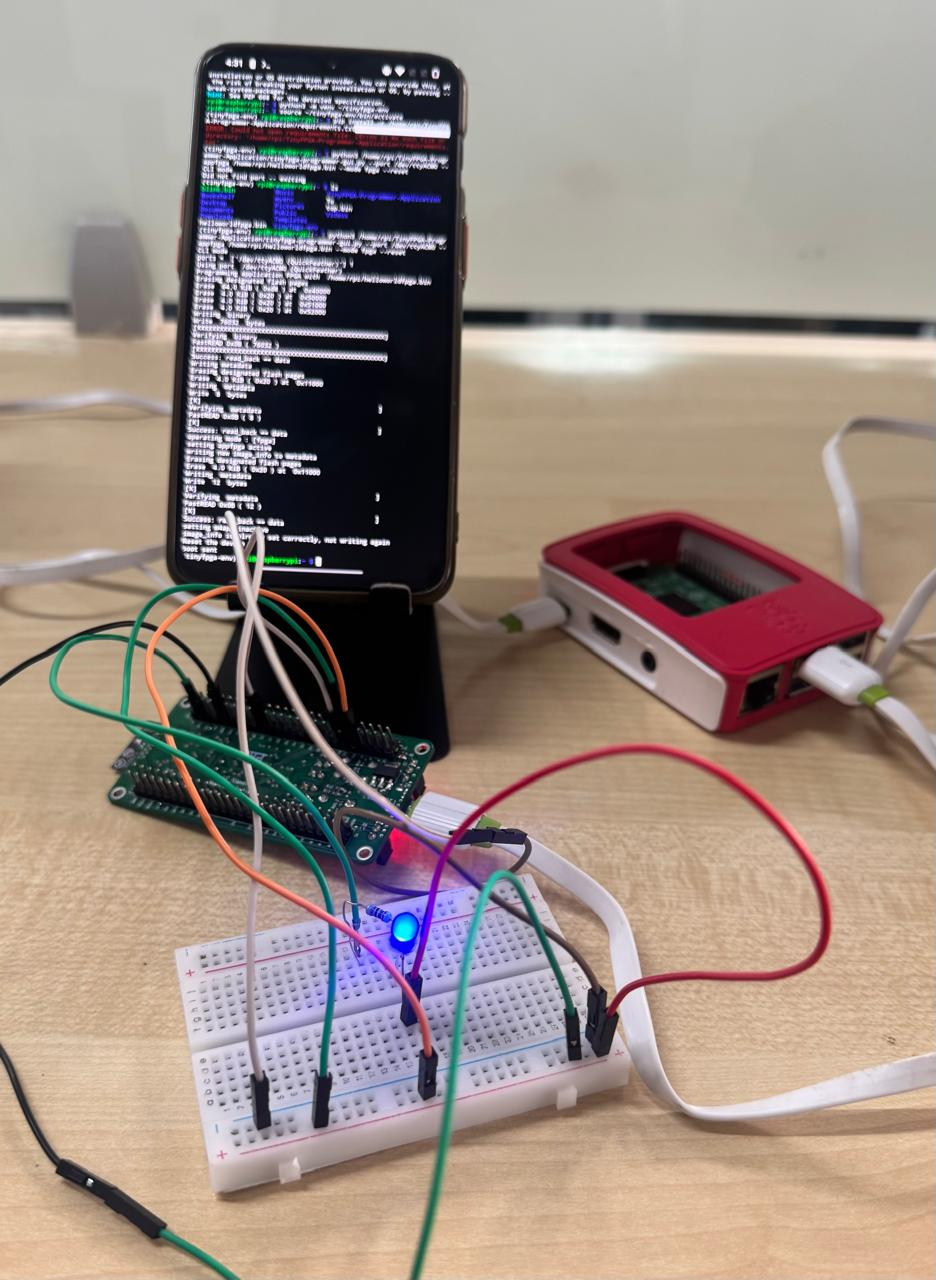
\includegraphics[width=0.4\textwidth]{/storage/emulated/0/FWC1/fpga/IMG-20241202-WA0012.jpg}
\end{figure}


\section{CONCLUSION}
 the project successfully implemented a Boolean logic circuit using the Raspberry Pi and pygm board to control an output based on the expression $B={\bar{D3}}D2+{\bar{D3}} {\bar{D1}}$,which was validated by the LED's on/off behavior. This demonstrated the effectiveness of Boolean algebra in hardware and how digital logic design circuits are responsive to input conditions. The project serves as a practical example of real-time logic processing, applicable to more complex digital systems and IoT applications.
\end{document}
